\documentclass[12pt,a4paper,openright,oneside]{article}
\usepackage{amsfonts, amsmath, amssymb,latexsym,amsthm, mathrsfs, enumerate}
\usepackage[catalan]{babel}
\usepackage{epsfig}

\parskip=5pt
\parindent=15pt
\usepackage[margin=1.2in]{geometry}
\usepackage{graphicx}
\usepackage{listings}
\usepackage[utf8]{inputenc}
\usepackage{fancyvrb}
\setcounter{page}{0}


\numberwithin{equation}{section}
\newtheorem{teo}{Teorema}[subsubsection]
\newtheorem*{teo*}{Teorema}
\newtheorem*{prop*}{Proposició}
\newtheorem*{corol*}{Corol·lari}
\newtheorem{prop}{Proposició}[subsubsection]
\newtheorem{corol}{Corol·lari}[subsubsection]
\newtheorem{lema}{Lema}[subsubsection]
\newtheorem{defi}{Definició}[subsubsection]
\newtheorem{nota}{Notació}

\theoremstyle{definition}
\newtheorem{prob}{Problema}
\newtheorem*{sol}{Solució}
\newtheorem{ex}{Exemple}
\newtheorem{exs}{Exemples}
\newtheorem{obs}{Observació}
\newtheorem{obss}{Observacions}

\def\qed{\hfill $\square$}

\renewcommand{\refname}{Bibliografia}
% --------------------------------------------------
\usepackage{fancyhdr}

\lhead{}
\lfoot{}
\rhead{}
\cfoot{}
\rfoot{\thepage}

\begin{document}

\bibstyle{plain}

\thispagestyle{empty}

\begin{titlepage}
\begin{center}
\begin{figure}[htb]
\begin{center}

\includegraphics[width=6cm]{ub.png}
\end{center}
\end{figure}

\textbf{\LARGE Treball final de grau} \\
\vspace*{.5cm}
\textbf{\LARGE GRAU EN ENGINYERIA INFORMÀTICA } \\
\vspace*{.5cm}
\textbf{\LARGE Facultat de Matemàtiques \\ Universitat de Barcelona} \\
\vspace*{1.5cm}
\rule{16cm}{0.1mm}\\
\begin{Huge}
\textbf{EINES BASADES EN TEXT PER A LA VISUALITZACIÓ I GEOLOCALITZACIÓ DE NOTÍCIES} \\
\end{Huge}
\rule{16cm}{0.1mm}\\

\vspace{1cm}

\begin{flushright}
\textbf{\LARGE Autor: Solanes Font, Aleix}

\vspace*{2cm}

\renewcommand{\arraystretch}{1.5}
\begin{tabular}{ll}
\textbf{\Large Director:} & \textbf{\Large Dr. Jordi Vitrià Marca} \\
\textbf{\Large Realitzat a:} & \textbf{\Large  Departament de Matemàtica Aplicada    } \\
 & \textbf{\Large i Anàlisi} \\
\\
\textbf{\Large Barcelona,} & \textbf{\Large \today }
\end{tabular}

\end{flushright}

\end{center}










\end{titlepage}


\newpage
\pagenumbering{roman} 

\section*{Abstract} 
This project came up after a few meetings with the professor Dr. Jordi Vitrià talking about Data Science, the possibilities inside this sector, about interesting projects that people made using Data Science, we talked about some cases that could be interesting to analyse, all with a spot in mind, the possibility of reaching a result and visualize that result in an understandable way. So, after those inspiring meetings we achieved the main idea of this project: Geolocation of news. \\ \\
Regarding the journalism sector, hundreds of news are published every day, but unfortunately not all of them include a proper geographic reference. All those news with a reference to a geographic location let the door open to a new way of distribution, and also let new ways of analysis based on this new parameter, the location. \\
As an example, imagine that a developer wants to let a user with a smartphone or a tablet, receive automatically the news related to the place where the user is. Without a reference to where the news took place it is difficult to face the problem, however with a reference to a place the problem now seems affordable.\\ \\
During the realization of this project, various tools and methods are used in order to obtain automatically a set of georeferenced tags from the news and thus be able to show the results in an easy way to analyse. \\
Despite being this project based in the concept of Data Science, I am not explicitly  using algorithms from the world of Data Science (in this report I will explain the reasons why some algorithms could not be used), I follow, however, the main principles: look for databases that can help me face the problem, clean all data in order to be able to use it, and finally I try to show the results in an understandable way to reach results or conclusions. \\ \\
This document outlined in detail the design, development and implementation of every single step that was necessary to achieve the final result.\\ \\
In order to see the results in a simple way, I also created a website with a summary of all the project and some visualizations of the results under the following URL:\\
http://alsolanes.github.io/TFG
\newpage
\section*{Resum}
Aquest projecte va néixer al cap d'algunes reunions amb el professor Dr. Jordi Vitrià en les quals parlàvem sobre Data Science i les seves possibilitats, sobre projectes interessants que la gent havia creat, sobre casos que seria interessant de poder analitzar, i tot amb una fita: la possibilitat d'arribar a algun resultat i fer que aquest es pogués representar visualment d'una forma entenedora. \\\\
En el sector del periodisme es publiquen centenars de notícies cada dia, però malauradament no totes elles inclouen la seva corresponent referència geogràfica. Que una notícia tingui aquesta referència, pot obrir nous camins en la distribució d'aquestes, així com permetre noves opcions d'anàlisi. Per exemple, considerem un desenvolupador que vol permetre a un usuari amb un smartphone o una tablet, que en funció d'on estigui, rebi les notícies automàticament d'aquesta zona. Sense cap referència a aquestes notícies seria difícil encara el problema, no obstant, si disposem d'aquesta informació el problema es simplifica.\\ \\
En el marc d'aquest projecte, s'utilitzaran diferents eines i mètodes per a poder obtenir d'una forma automàtica les referències geogràfiques d'un conjunt de notícies i així poder-ne representar els resultats d'una forma que sigui senzilla d'analitzar posteriorment.\\
Aquest projecte neix de la curiositat que em despertava el món de la Data Science, o més concretament, el poder acabar extraient conclusions d'una sèrie de dades. Si bé no s'utilitzen explícitament algorismes pròpiament del món de Data Science (durant aquesta memòria s'explicaran els motius pels quals alguns algorismes no s'han pogut utilitzar), si que es segueixen les idees fonamentals d'agafar una gran quantitat de dades, netejar-les i finalment mirar de visualitzar les dades per a facilitar la tasca d'obtenció de resultats o conclusions.\\ \\
Per tal de facilitar l'accés als resultats també s'ha habilitat una pàgina web amb el procés resumit així com la visualització dels diferents resultats obtinguts. La direcció en qüestió és:
\begin{quote}
\centering
http://alsolanes.github.io/TFG
\end{quote}

\newpage 


\section*{Agraïments}

Vull agrair a ... 
\newpage

\tableofcontents

\newpage

\pagenumbering{arabic} 
\setcounter{page}{1}
\section{Introducció}
Uns dies abans d'escollir el projecte, vaig tenir l'oportunitat de reunir-me amb el Dr. Jordi Vitrià, per tal de parlar sobre les possibilitats i temes en general relacionats amb Data Science. Durant aquestes converses, van sorgir diferents conceptes, diferents projectes que s'havien realitzat al voltant del món de la Data Science, així com idees que alimentaven la idea de que aprofitant l'oportunitat d'escollir un treball final de grau, seria una bona idea experimentar lleugerament amb algun projecte que hi estigués relacionat.\\
Abans d'introduir el projecte, però, introduiré els conceptes de Big Data i Data Science, ja que en són les arrels.
\subsection{Big Data}
Amb l'evolució de les tecnologies de la informació, s'ha incrementat també la quantitat de dades que es produeixen a internet. En plantejar-se com tractar tota aquesta nova quantitat d'informació, es va veure que per exemple no era viable carregar totes aquestes dades en una base de dades relacional per al seu anàlisis. D'aquesta manera, va aparèixer el concepte de Big Data, per a fer referència a tota aquella informació que no pot ésser processada o analitzada utilitzant processos o eines que hi havia fins aleshores.\\
\subsection*{Quins tipus de dades es poden generar?}
Aquesta gran quantitat d'informació pot venir de diferents fonts, i fins i tot s'ha de tenir en compte que no només aquesta informació és generada pels humans, sinó que existeixen dades creades per màquines, com pot ser el cas de les M2M (Machine-to-Machine).
\begin{figure}[htbp]
\centering
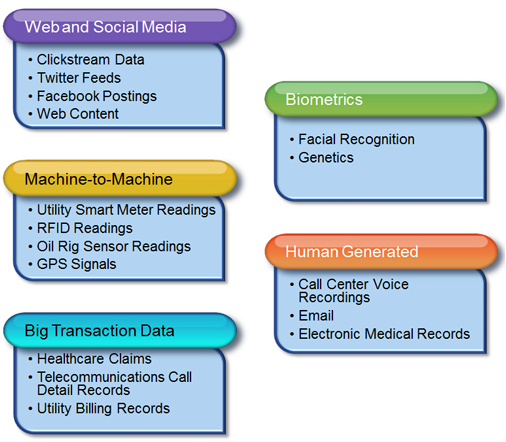
\includegraphics[width=6cm]{tipus_data.png}
\caption{Tipus de dades a analitzar dins el sector Big Data.}
\end{figure}
Tipus de dades:
\begin{itemize}
\item \textbf{Web i xarxes socials}: Es tracta de la informació generada en pàgines web, així com les dades obtingudes a través de les Xarxes Socials.
\item \textbf{Machine-to-Machine(M2M)}: Són les tecnologies que permeten la interconnexió entre dispositius. S'utilitzen dispositius com ara sensors o mesuradors per a generar dades, i fer que un altre màquina pugui interpretar aquestes dades i donar-los-hi sentit.
\item \textbf{Big Transaction Data}: Són dades transaccionals, disponibles tant de forma semiestructurada com no estructurada. Entre els tipus de dades que inclou, s'hi troben per exemple registres de facturació o registres detallats de trucades (CDR).
\item \textbf{Biomètriques}: Són dades biomètriques que inclouen informació sobre empremtes dactilars, escanejos de retina, reconeixement facial, genètica, etc. Són dades especialment importants en els sectors de seguretat. 
\item \textbf{Dades generades per humans}: És la informació que generem al enviar correus, escriure documents electrònics, en fer-nos estudis mèdics, deixar missatges de veu,... 
\end{itemize}
I dins tota aquesta quantitat d'informació hi podríem incloure també la que pot generar una empresa de premsa, la qual genera centenars de notícies a diari amb les seves respectives meta-dades, les imatges, vídeos, i tota la informació que correspongui a cada notícia.\\\\
Una vegada tenim totes aquestes dades, és necessari un tractament per a poder mirar d'entendre i extreure'n conclusions, i és aquí on entra el món de la Data Science.
\subsection{Data Science}
Data Science, és un nou camp que està estretament lligat amb l'anàlisi de Big Data, però no es centra exclusivament en projectes de Big Data, ja que l'objectiu principal és l'extracció de coneixement d'una font de dades.

\begin{quote}
\emph{"A Data scientist is somebody who is inquisitive, who can stare at data and spot trends. It's almost like a Renaissance individual who really wants to learn and bring change to an organization."}
\begin{flushright}
- Anjul Bhambhri, vicepresident dels productes Big Data d'IBM.
\end{flushright}
\end{quote}

Les persones que treballen en Data Science, s'anomenen Data Scientists, i la seva formació es basa en tres grans eixos: coneixement del negoci, capacitats en programació, i formació en matemàtiques i estadística.

\begin{figure}[htbp]
\centering
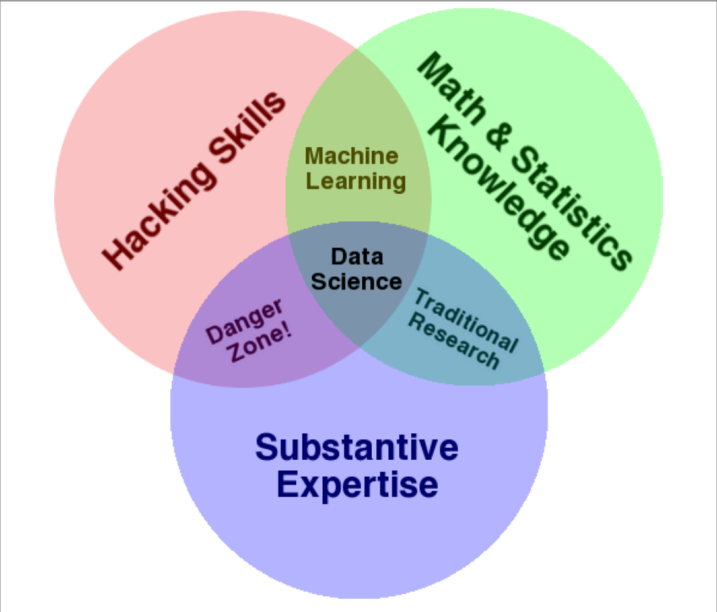
\includegraphics[width=6cm]{conway-datascience.png}
\caption{Diagrama de Venn de Data Science. De Drew Connway.}
\end{figure}
\newpage
Segons Nathan Yau, doctor en estadística per la universitat de UCLA i redactor cap del portal divulgatiu www.flowingdata.com, un expert en Data Science ha de tenir les següents capacitats:
\begin{itemize}
\item Estadística
\item Data munging: capacitat per a manipular i adaptar les dades segons les necessitats (parsing, scraping i formatting data).
\item Visualització de les dades (graphs, mapes,...).
\end{itemize}
L'aparició del terme Data Science, té els seus orígens en els requeriments que demanava per algunes ofertes de feina Google, i que demanaven les següents habilitats per als futurs candidats:
\begin{quote}
\emph{"...working with a team on problems that require a hybrid skill set of stats and computer science paired with personal characteristics including curiosity and persistence."}
\begin{flushright}
- Fragment d'una oferta de feina de l'any 2008 abans de l'acceptació del terme Data Science.
\end{flushright}
\end{quote}
Veient que existia la creixent demanda d'aquest perfil, el Dr. Dhanurjay "DJ" Patil juntament amb Jeff Hammerbacher (Facebook i LinkedIn respectivament) van decidir encunyar el terme "Data Science" per a descriure aquest lloc de treball. 
\newpage
\subsection{El projecte}

El següent projecte es centra en l'anàlisi d'un conjunt de notícies, i obtenir de cada notícia un o varis punts geogràfics que representaran l'àmbit geogràfic d'on està parlant el text, per a posteriorment mostrar en un mapa els resultats d'aquest anàlisi.\\ \\
Per a poder arribar aquests resultats el procés es divideix en quatre grans etapes:
\begin{enumerate}
\item Recopilació de notícies
\item Cerca i neteja d'una base de dades fiable que contingui noms de localitats i les seves coordenades.
\item Anàlisi del text de cada notícia recopilada per a extreure'n noms de ciutats.
\item Representar les localitats trobades en un mapa.
\end{enumerate}

Totes aquestes etapes s'aniran detallant en el desenvolupament del següent document.\\
Una vegada es tinguin els resultats, els mapes resultants així com una explicació general del procés per arribar-hi, estarà disponible mitjançant una pàgina web pública, des de la qual es posarà el codi a disposició del públic.

\subsection{Antecedents}
\subsection*{Yahoo BOSS Geo Services}

\begin{figure}[htbp]
\centering
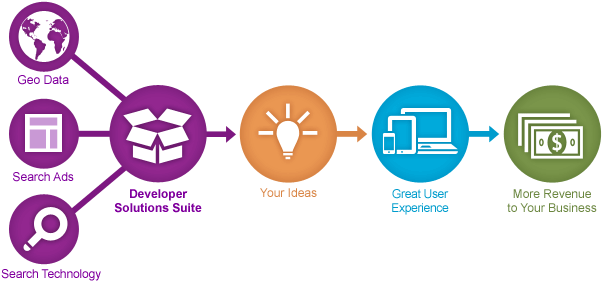
\includegraphics[width=6cm]{Yahoo_boss.png}
\caption{Esquema de negoci de Yahoo BOSS}
\end{figure}
Yahoo BOSS Geo Services, és un servei web que es divideix en dos projectes:
\begin{itemize}
\item PlaceFinder: Permet als seus usuaris trobar les coordenades concretes d'una direcció o localitat.
\item PlaceSpotter: Donat un text que pot pertànyer a un twit de twitter, una notícia, una pàgina web, entre altres, retorna les localitats que ha pogut localitzar dins d'aquest text.
\end{itemize}
És un servei de pagament, i el seu cost varia en funció del nombre de queries diàries que es desitgin fer.
\subsection*{CLAVIN}
\begin{figure}[htbp]
\centering

\includegraphics[width=6cm]{clavin.png}
\caption{Logotip del projecte CLAVIN.}
\end{figure}
CLAVIN (Cartographic Location And Vinicity INdexer) és un projecte open source que té com a objectiu assignar "tags" a un document d'entrada especificant la geolocalització d'aquest text. Per a analitzar el text, combina diferents eines open source per a aplicar un processament de llenguatge natural i finalment, amb l'ajut d'un Gazeteer
\footnote{Diccionari geogràfic que conté correspondències entre informació geoespacial i noms.},
 poder trobar les paraules referents a punts geogràfics correctament. Està especialitzat amb treballar sobre grans quantitats d'informació, Big Data, i és per això que per a processar aquestes grans quantitats de dades utilitza el framework Hadoop\footnote{Framework de software que permet treballar amb milers de nodes i amb petabytes de dades.}.\\\\
Com a exemple de funcionament, aprofitarem que la seva pàgina web permet testejar la seva aplicació (http://clavin.berico.us/clavin-web/), agafarem un text qualsevol en anglès (en qualsevol altre idioma no funciona).\\
El text parla sobre un edifici de Portsmouth que el volen pintar dels colors de l'equip rival de futbol de la ciutat, i d'on a simple vista es poden localitzar com a ciutats d'on parla la notícia les ciutats de Portsmouth, Hampshire i Southampton.
\begin{figure}[htbp]
\centering
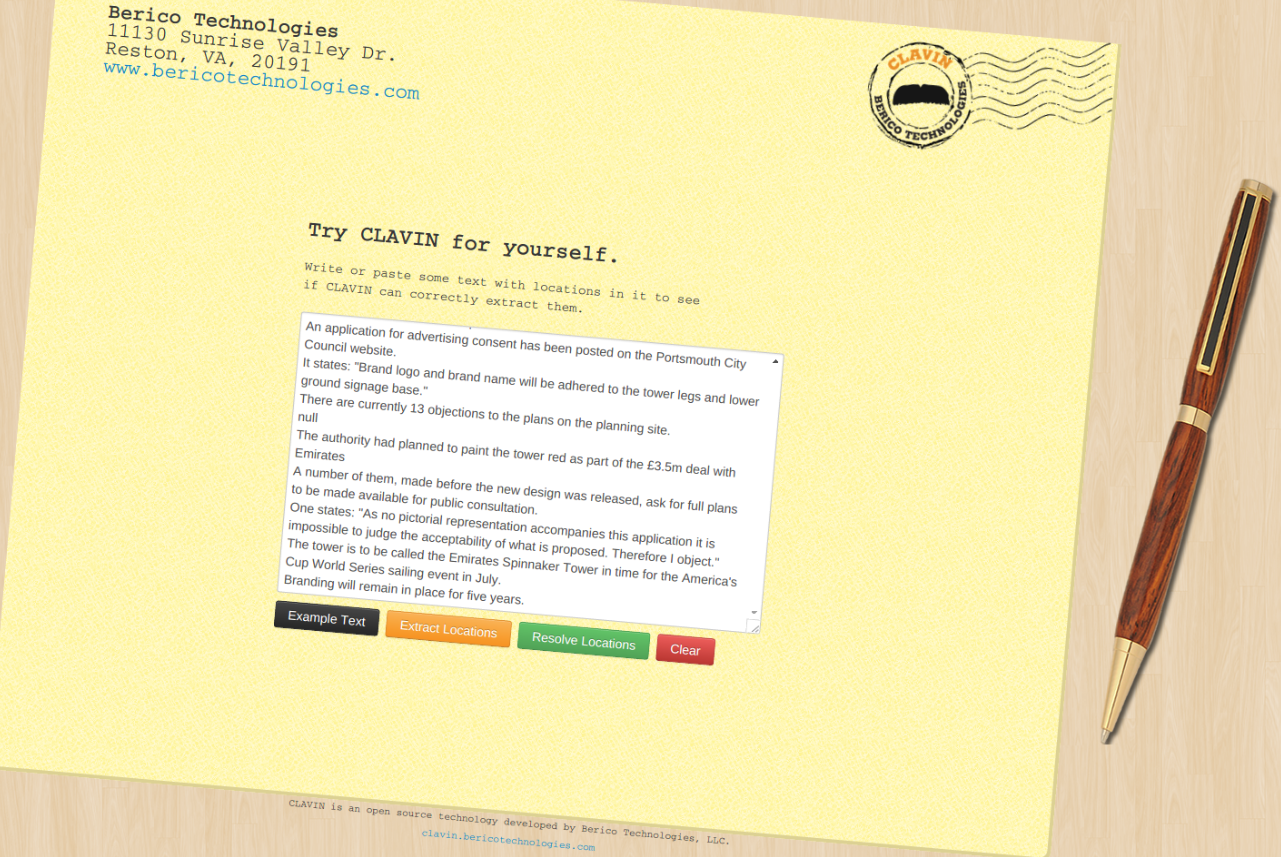
\includegraphics[width=7cm]{clavin-1.png}
\caption{Pàgina web que permet testejar el funcionament del parsejador de punts geogràfics.}
\end{figure}
\begin{figure}[htbp]
\centering
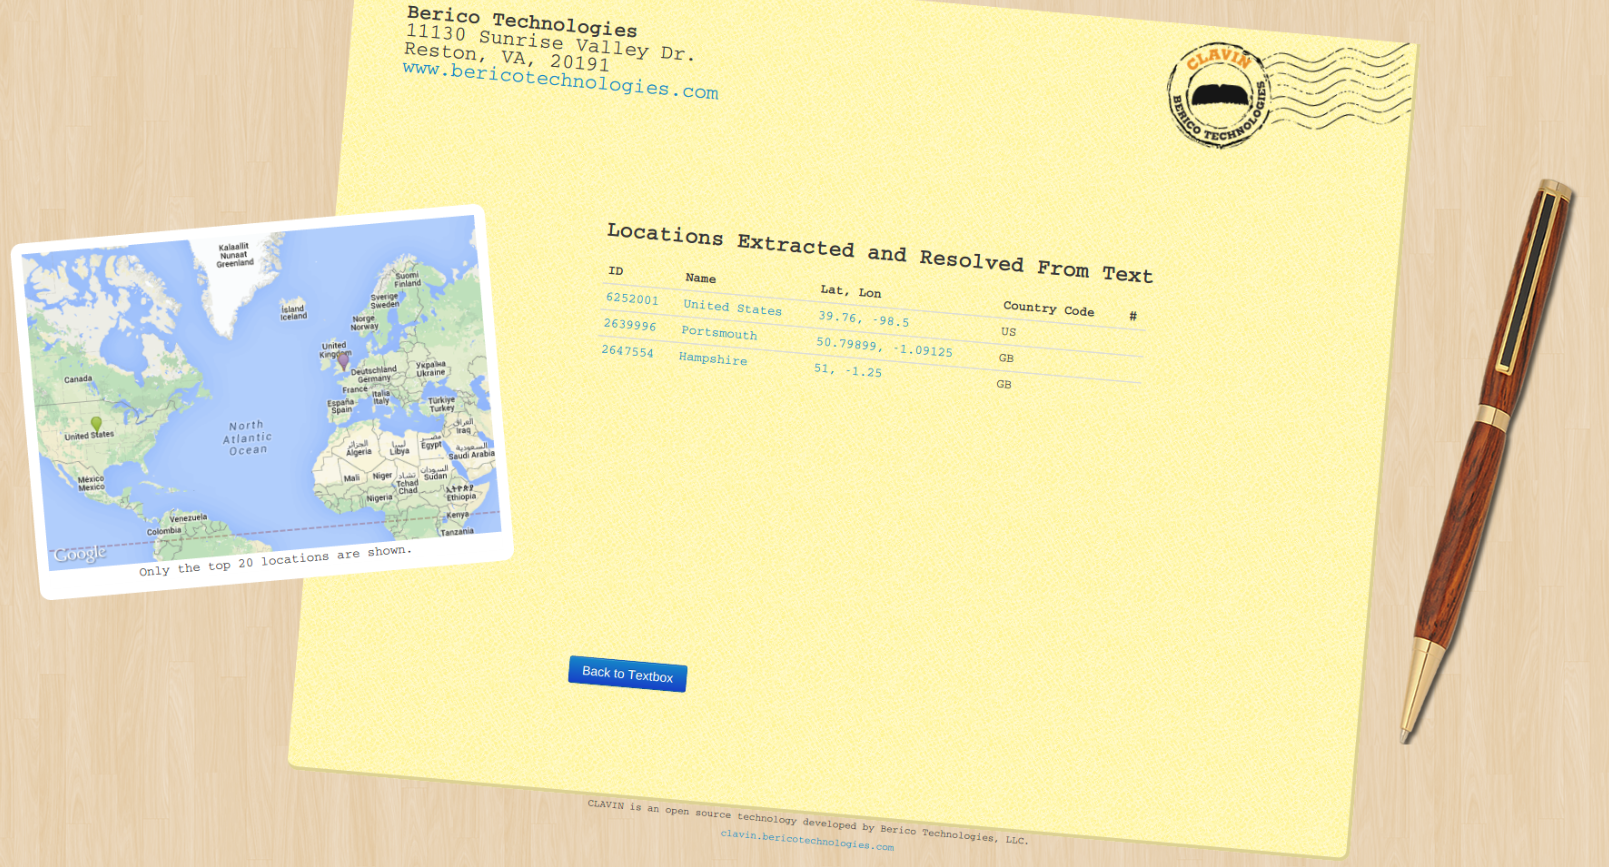
\includegraphics[width=7cm]{clavin-2.png}
\caption{Pàgina web que mostra a la part esquerra un mapa amb les ciutats trobades, i a la dreta la llista de ciutats junt amb les seves coordenades i el país.}
\end{figure}Podem comprovar com els resultats que ens indica són les ciutats de Portsmouth i Hampshire, mentre que no ha posat la ciutat de Southampton, donat que la notícia en general no parla de Southampton i només ho menciona pel seu equip de futbol. També posa com a resultat els Estats Units en general.
\newpage
\subsection*{TextGrounder}
TextGrounder és un projecte que pretén trobar mencions en un text sobre llocs geogràfics o referències temporals. Per a poder retornar la informació correctament, utilitza mètodes de processat de llenguatge natural (NLP) juntament amb algorismes de machine learning per a analitzar el context de la paraula i fer més fiable el resultat donat.
Aquest projecte va néixer al setembre de l'any 2010 de les mans de Jason Baldridge (Universitat d'Austin) amb la intenció d'analitzar les referències temporals i geogràfiques en textos acadèmics del segle XIX.\\
Actualment està compost de tres subprojectes:
\begin{itemize}
\item Geolocalització de documents: Identifica la localització d'un document fent servir bases de dades d'entrenament, els quals contenen distribucions d'unigrames o bigrames que serveixen per a caracteritzar un text. Els textos utilitzats per a entrenar la base de dades principalment són textos de la Wikipedia.
\item Geolocalització de topònims: Desambigua cada topònim d'un document, crea un model estadístic per a caracteritzar el text, igual que en l'anterior subprojecte, però en aquest cas s'utilitza un gazeteer per a verificar aquests topònims.
\item Generador KML: Genera una sèrie de fitxers KML que contindran informació estadística sobre una sèrie de paraules, identificant per exemple les paraules més utilitzades al parlar d'una regió concreta de la terra.
\end{itemize}
\subsection*{Google Maps API}
La informació basant-se amb la base de dades dels seus mapes, està disponible a través d'aquesta API. Google ofereix dues versions de la API, una lliure i la versió "for work". La primera és una versió limitada, que ens permet realitzar un màxim de 2500 queries per dia i el projecte on s'utilitzi ha de ser gratuit per a tots els públics.
La seva utilització es basa en fer crides a un webservice passant-li una sèrie de paràmetres. Així per exemple si desitgem les coordenades d'una direcció concreta, fariem:\\
\begin{figure}[htbp]
\begin{verbatim}
https://maps.googleapis.com/maps/api/geocode/json?
address=585+Gran+Via+de+les+Corts+Catalanes,+Barcelona+,+ES&key=API_KEY
\end{verbatim}
\caption{Crida al webservice de la API de Google}
\end{figure}
\\
Aquesta crida, ens retornaria una resposta JSON la qual contindria informació sobre aquesta direcció, informant-nos del tipus d'edifici que es tracta, la latitud i la longitud.\\

\subsection{Estructura de la Memòria}
La següent memòria estarà estructurada de forma que primer s'explicaran els \textit{objectius i la definició del problema} per tal de tenir clar quina és la finalitat del treball. \\\\
A continuació es detallaran les diferents etapes de disseny i desenvolupament fins a arribar al resultat final. També es mencionaran aproximacions alternatives a la realització del problema que s'han intentat durant la realització del projecte. Aquesta informació estarà a la secció de \textit{Desenvolupament}.\\\\
A continuació, a la secció \textit{Metodologia i resultats}, es parlarà sobre les metodologies utilitzades durant la realització d'aquest projecte, així com les correspondències entre els resultats esperats, i els resultats reals.\\\\
Finalment, en l'apartat de \textit{Conclusions i vies de continuació}, s'analitzarà el resultat final del treball, i es detallaran les possibles futures ampliacions que es podrien fer al treball, així com possibles solucions per a reduir les limitacions que s'han trobat durant la realització del projecte.

\newpage

\section{Definició d'objectius i motivació del problema}
\subsection{Objectius}
Aquest projecte té com a principal finalitat permetre identificar els punts geogràfics on una notícia té lloc. Però per a poder arribar a aquest punt, s'han d'assolir una sèrie d'objectius on cada un d'ells té un pes igualment important per a poder obtenir uns resultats fiables. Els principals objectius marcats durant el projecte són:
\begin{enumerate}
\item Recopilar una sèrie de notícies per a poder ser analitzades
\item Crear una base de dades fiable amb les localitats que es tindran en compte per a la geolocalització de les notícies.
\item Permetre identificar, donat un text, les paraules que són susceptibles de ser una localitat.
\item Fent servir les bases de dades anteriors, mostrar en un mapa els diferents punts trobats, per a mostrar tant la evolució temporal, com el nombre total d'aparicions d'una localitat en les notícies.
\item Crear una pàgina web per a mostrar-ne els resultats, així com a permetre que altres usuaris puguin continuar o analitzar el desenvolupament.
\end{enumerate}
\subsection{Problema}
En el sector del periodisme, es publiquen centenars de notícies cada dia. Per exemple, la font de referència utilitzada, el diari Ara en la seva versió digital, crea al voltant de 120 notícies diàries.\\
Cada una d'aquestes notícies conté una sèrie de "tags", no obstant, aquestes paraules no sempre segueixen un ordre lògic, o senzillament no permeten categoritzar les notícies segons la seva ubicació geogràfica.
\subsubsection{Cicle de vida d'una notícia}
El cicle de vida d'una notícia conté tres grans etapes:
\begin{itemize}
\item Producció
\item Distribució
\item Consum
\end{itemize}
\newpage
\subsubsection*{Producció d'una notícia}
Durant la producció, és el procés en què el periodista crea la notícia, l'escriu i li assigna una sèrie de paraules que permetran identificar aquesta notícia. Aquestes paraules, poden ser noms de persona que hi apareixen, noms d'empresa, alguna paraula clau,... però no necessàriament ha de contindre la localitat d'on s'està parlant, donat que sovint resta a disposició del periodista assignar les paraules que ell cregui rellevants per al text que ha escrit.\\
\subsubsection*{Distribució d'una notícia}
En aquesta etapa, la notícia ja ha estat creada, revisada, se li han assignat unes paraules clau, s'ha introduït a la base de dades del diari, i ja està en el punt de quedar a la disposició dels clients o usuaris que desitgin accedir a aquesta notícia. La distribució es pot fer en físic o en digital, tot i que en el nostre cas ens centrarem en la part digital. Aquesta distribució es sol realitzar a través de mètodes de distribució com ara RSS (Really Simple Syndication), a través de la seva pàgina web, o d'alguna aplicació mòbil.\\
\subsubsection*{Consum d'una notícia}
Finalment, l'usuari té la notícia a la seva disposició i la pot estar consultant. En aquesta etapa, no hi intervé res més que l'usuari, la notícia en sí i el terminal des d'on l'estigui consumint, ja que qualsevol etapa extra com podria ser el fet que s'ordeni o categoritzi les notícies es consideraria dins l'etapa de distribució d'aquesta.
\\\\
Aquest projecte pretén ser una ajuda per a les etapes de producció (permetent per exemple ajudar a l'escriptor de la notícia a localitzar paraules susceptibles de ser localitats mencionades en la notícia), i per la distribució (permetent tenir les notícies categoritzades segons la zona geogràfica on té lloc la notícia).
\newpage
\section{Desenvolupament}
Per al procés de desenvolupament del projecte he fet servir diferents eines que m'han facilitat les diferents etapes del procés, cada tecnologia utilitzada facilita una aproximació al problema, és per això, que també és interessant mencionar altres tecnologies que he pogut experimentar durant aquest projecte, tot i que finalment pot ser que no els hagi utilitzat per l'aproximació final. Tot seguit en presento primer les tecnologies utilitzades, i a continuació altres tecnologies que facilitarien una diferent visió del problema.
\subsection{Eines utilitzades}
\subsection*{Github}
\begin{figure}[htbp]
\centering

\includegraphics[width=7cm]{github.jpg}
\caption{Logotip de Github.}
\end{figure}
És una eina que bla bla...\\
flkj
\subsection*{Python}
\begin{figure}[htbp]
\centering

\includegraphics[width=7cm]{python.png}
\caption{Logotip de python.}
\end{figure}
És una eina que bla bla...
\newpage
\subsection*{IPython}
\begin{figure}[htbp]
\centering
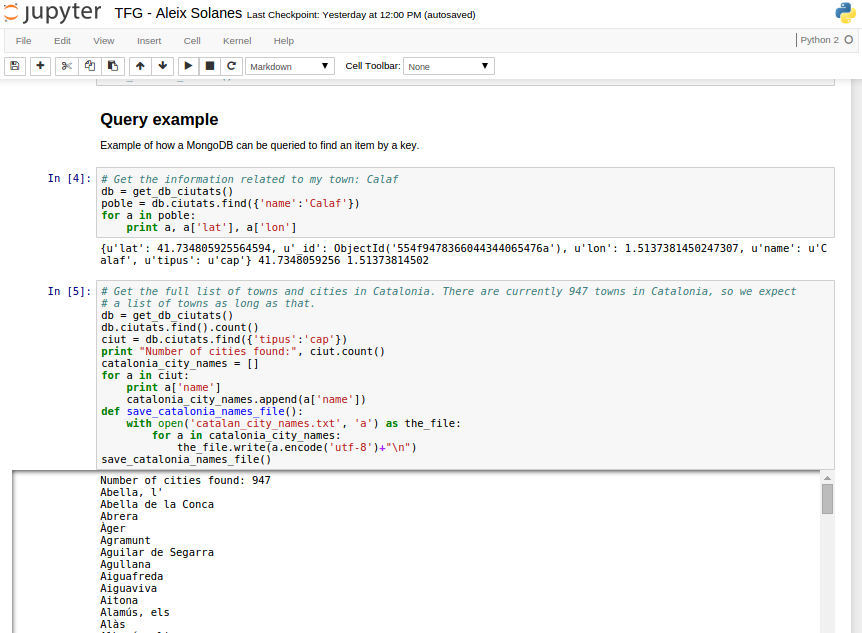
\includegraphics[width=9cm]{ipython.png}
\caption{Exemple d'una notebook d'IPython.}
\end{figure}
\subsection*{RSS}

\subsection*{MongoDB}

\subsection*{JSON}

\subsection*{CartoDB}

\subsection{Fonts de les dades}

\subsection*{RSS - Diaria Ara, Vilaweb, Regió7}

\subsection*{Geonames}

\subsection*{ICC - Institut Cartogràfic de Catalunya}

\subsection*{Github.io}

\subsection{Una visió alternativa, altres eines}

\subsection*{NLP (Natural Language Processing)}

\subsection*{NER (Named-Entity Recognition}

\subsection*{SPARQL}

\subsection{Preparació de l'entorn MongoDB i conceptes bàsics}
Per a la gestió de les bases de dades que s'han utilitzat en el projecte, s'utilitzarà una aproximació NoSQL, MongoDB. Utilitzar una base de dades NoSQL no és una elecció que s'hagi pres sense motiu, ja que es buscava una escalabilitat i una agilitat que una base de dades relacional SQL clàssica no facilitava uns resultats tan bons.\\
En definitiva el que es necessita és, partint d'un model clau-valor, fer cerques ràpides que retornin un valor al especificar una clau, i en això, els models NoSQL són idonis. Més concretament, MongoDB emmagatzema les seves bases de dades en format BSON (Binary JSON). BSON és una serialització amb codificació binària d'una sèrie de documents amb format JSON. Cada document o objecte, és el que es podria considerar com una espècie d'equivalent del que es coneix com a taula amb termes SQL. \\ \\
Així doncs, una vegada definit l'entorn que s'utilitzarà per a la gestió de les bases de dades, es procedeix a la seva inicialització. La qual en un entorn python ens resultarà especialment simple fent servir la llibreria \emph{PyMongo}. Una vegada s'ha engegat el servidor de la base de dades, que per executar-lo en un entorn Linux s'ha d'executar la comanda "\emph{sudo mongod}", la inicialització bàsica és tan simple que amb dues línies de codi Python permet deixar apunt per a ser utilitzada la nostra base de dades.:

\begin{figure}[!htbp]
\begin{verbatim}
client = MongoClient('localhost:27017')
db = client.ciutats
\end{verbatim}
\caption{Inicialització d'una base de dades MongoDB amb la llibreria PyMongo.}
\end{figure}
Ara que ja es té inicialitzada la base de dades, afegir una ciutat amb les seves corresponents dades, serà fer un insert com el següent:

\begin{figure}[!htbp]
\begin{verbatim}
db.ciutats.insert({"name":name, "tipus":tipus,"lat":lat, "lon":lon})
\end{verbatim}
\caption{Insert a una base de dades utilitzant PyMongo.}
\end{figure}
On "\emph{name}" serà el nom del camp, i \emph{name} el seu valor.\\ \\
Per a poder fer consultes sobre una base de dades MongoDB, es pot utilitzar la comanda find de la llibreria PyMongo.

\begin{figure}[htbp]
\begin{verbatim}
db.ciutats.find({'name':'Calaf'})
\end{verbatim}
\caption{Exemple de consulta bàsica utilitzant PyMongo.}
\end{figure}
Com podem veure en la figura anterior, per a fer una consulta bàsica utilitzant l'instrucció find, només cal que especifiquem quin camp estem buscant i el valor concret d'aquest. En aquest cas la consulta ens retornaria una estructura JSON amb la informació disponible per al municipi de Calaf com la següent:
\begin{figure}[!htbp]
\begin{verbatim}
{u'lat': 41.734805925564594, u'_id': ObjectId('554f947836604436a'), 
u'lon': 1.5137381450247307, u'name': u'Calaf', u'tipus': u'cap'}
\end{verbatim}
\caption{Exemple de resposta d'una consulta bàsica utilitzant PyMongo.}
\end{figure}
\newpage
\subsection{Obtenció i neteja de les dades}
La primera etapa del procés de desenvolupament del projecte, ha estat la cerca de les bases de dades corresponents que d'una forma fiable pugui permetre arribar a uns resultats acceptables. És una de les etapes del projecte més importants, donat que qualsevol resultat que se'n desprengui depèn estrictament d'aquestes dades. Per a poder trobar la base de dades final se n'han hagut de provar unes quantes, i fer la corresponent recerca. Fins i tot s'han intentat desenvolupaments alternatius per a construir manualment les bases de dades, com s'explica en la secció de \textit{desenvolupaments alternatius}.\\ \\
En aquesta secció, s'explicarà els processos seguits per tal d'\emph{obtenir}, \emph{analitzar}, i \emph{processar} totes les bases de dades utilitzades en el projecte, per tal de en la següent etapa poder-les utilitzar sense problemes, considerant que hi haurem deixat només la informació important, i en el cas que sigui necessari haurem adaptat el format d'algunes dades per a facilitar la seva utilització.\\ \\
En la introducció, hem parlat sobre el terme Data Science. Si recordem les tres habilitats que el Dr. Nathan Yau mencionava com a pilars en qualsevol Data Scientist (Estadística, Data munging i Visualització de les dades), aquesta etapa faria referència al terme "\emph{Data munging}". Aquest terme, ve del verb en anglès "Munge", el qual significa "transformar dades d'una forma indefinida".
\subsubsection*{D'on extreure les bases de dades?}
En aquest projecte, s'han utilitzat dues aproximacions per a l'obtenció de les bases de dades. Una és senzillament buscar una font fiable i descarregar-la, com en el cas de les ciutats i els seus punts geogràfics; l'altra, donada la impossibilitat de trobar de forma senzilla una base de dades que s'ajustés a les necessitats, ha estat crear-la, buscant un lloc d'on extreure les dades i emmagatzemant-la en una base de dades pròpia, com en el cas de l'obtenció de les notícies a analitzar.
\subsubsection*{Perquè modificar les bases de dades obtingudes?}
S'ha de tenir present, que quan es facilita una base de dades, se'n sol especificar el format per tal que qualsevol persona que la vulgui utilitzar sàpiga com tractar-la. Per desgràcia, cada llenguatge pot tenir les seves particularitats alhora de tractar amb dades, i per això pot ser necessari donar un format concret a les dades prèviament obtingudes. \\També s'ha de tenir en compte, que una base de dades pot incloure molta informació que de bon principi ja se sap que no és necessària per a la implementació d'un projecte, i en aquests casos, per temes d'agilitat i d'espai, també pot ser interessant destriar-ne aquella que resulti innecessària.


\newpage
\subsection*{Base de dades de pobles i ciutats de Catalunya}
Per tal d'obtenir uns resultats el més bons possible, és molt important que les bases de dades que s'utilitzin continguin informació el màxim de fiable. És per això, que després de que s'hagin investigat i provat diferents alternatives, s'ha decidit optar per una base de dades facilitada per l'Institut Cartogràfic de Catalunya, la qual inclou més de 52.000 referències geogràfiques del territori català. Aquesta base de dades està disponible al públic sota el següent enllaç:
\begin{quote}
http://www.icc.cat/index.php/Home-ICC/Publicacions/Nomenclator
\end{quote}
Aquesta informació, que s'ha definit com a base de dades, en un principi és considerat un Nomenclàtor. Aquest terme, fa referència a un document amb informació sobre un nucli poblacional, que pot ésser inferior a una unitat poblacional com pot ser el municipi (nucli de població, llogarets, parròquies,...), i en detalla informació sobre en quina forma s'hi assenta la població. A més, en facilita informació geogràfica, com ara les seves coordenades, cosa que és el que més interessa per a la realització del treball.\\
El primer pas abans de prosseguir és veure quins diferents tipus de dades inclou aquesta base de dades.

\begin{table}[htbp]
\begin{center}
	\centering
    \begin{tabular}{| l | l | l | l |}
    \hline
    \textbf{Abreviació} & \textbf{Significat} \\ \hline
    'cap' & Cap de municipi \\ \hline
	'barri' & Barri, sector urbà (superior a 50.000 habitants)\\ \hline
	'nucli' & Nucli de població(poble, llogaret...)\\ \hline
	'diss.' & Veïnat disseminat \\ \hline
	'e.m.d.' & Entitat municipal descentralitzada \\ \hline
	mun. & Nom del municipi quan aquest no coincideix amb la capital \\ \hline
	edif. & Edificació aïllada\\ \hline
	edif. hist. & Edifici històric (ermita, església, castell,...)\\ \hline
    \end{tabular}
\end{center}
\caption{Tipus de dades inclosos en el nomenclàtor del ICC.}
\end{table}
Es pot veure doncs, que el que interessa més per aquest projecte és el terme 'cap', que fa referència a Cap de municipi. Per a comprovar que és el que s'entén com a municipi, senzillament es comprova que hi ha 947 referències sota el terme 'cap.', el mateix nombre exacte de municipis que es troben registrats a Catalunya.
\subsubsection*{Estructura de les dades}
El document que inclou tota la informació del nomenclàtor, és un document en format .xlsx (document específic del programa Microsoft Excel, a partir de la seva versió 2007). Per tant, el primer pas en obtenir unes dades, és veure'n el format, per a saber com encarar la seva refactorització per a poder utilitzar-la en el projecte.
\newpage
\begin{figure}[htbp]
\centering
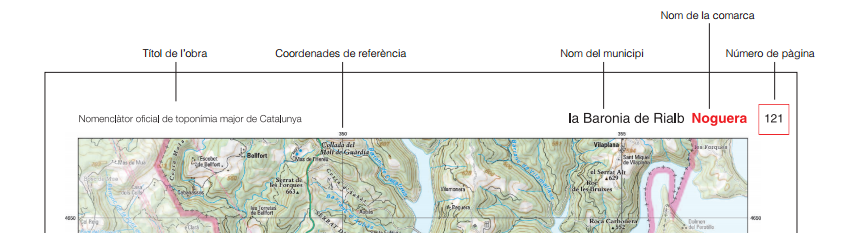
\includegraphics[width=15cm]{nomenclator.png}
\caption{Nomenclàtor oficial de toponímia major de Catalunya.}
\end{figure}
Aquest fitxer d'Excel, fa referència al nomenclàtor oficial de toponímia major de Catalunya, una obra que inclou informació concreta per a cada municipi de Catalunya. És per això que en els termes que analitzarem a continuació hi podem trobar camps de referència a aquesta obra, com ara els camps Volum o el camp pàgina, que indiquen la localització dins la obra física del municipi especificat.\\
Anem a veure les diferents columnes del fitxer d'Excel:
\begin{itemize}
\item \textbf{Topònim}: Nom del punt geogràfic.
\item \textbf{Concepte}: Tipus d'assentament poblacional ('cap', nucli, barri, diss.,...)
\item \textbf{Municipi 1}: Indica el municipi al qual pertany el topònim en qüestió, inclou 4 camps (Municipi 1, Municipi 2, Municipi 3, Municipi 4) a la taula, que indiquen el cas en que pugui pertànyer a múltiples municipis.
\item \textbf{Comarca 1}: Indica a la comarca que pertany el topònim. Pot pertànyer a fins a 5 comarques, per tant inclou 5 camps (Comarca 1, Comarca 2, ..., Comarca 5).
\item \textbf{UTM X i UTM Y}: Coordenades X i Y en el Sistema de Coordenades Universal Transversal de Mercator.
\item \textbf{Volum}: Indicador que fa referència al volum físic de l'obra (Nomenclàtor Oficial de toponímia major de Catalunya).
\item \textbf{Pàgina}: Indicador que fa referència a la pàgina dins el volum físic de l'obra.
\item \textbf{UTMX i UTMY}: Coordenades precises X i Y en el Sistema de Coordenades Universal Transversal de Mercator.
\end{itemize}
\begin{figure}[htbp]
\centering
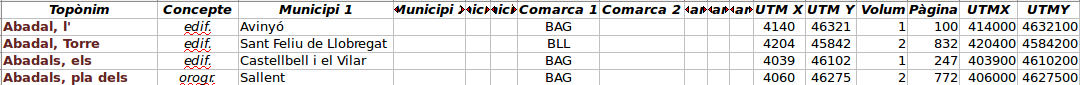
\includegraphics[height=2cm,width=16cm]{nomenclator_taula.png}
\caption{Nomenclàtor oficial de toponímia major de Catalunya.}
\end{figure}
\subsubsection*{Neteja}
Ara que ja sabem el format que tenen les dades, ja podem iniciar el procés per a extreure la informació que ens interessa i deixar-la apunt per a ésser manipulada.\\
Per a fer aquest procés utilitzarem la llibreria \emph{xlrd} per a python, la qual ens permet la manipulació de fitxers amb dades procedents del Microsoft Excel, més concretament ens permet l'extracció de dades de fitxers d'Excel .xls i .xlsx a partir de la versió 2.0.\\ \\
De totes les dades que disposa la base de dades, es conservaran les dades referents al nom del municipi (columna "Topònim"), al tipus de municipi (columna "Concepte") i les seves coordenades geogràfiques corresponents a les columnes UTMX i UTMY.\\
Per a les dades corresponents a les coordenades, es convertiran aquestes dades al sistema de coordenades esfèriques, on mantindrem els paràmetres de latitud i longitud en la nostra base de dades.
\subsubsection*{Conversió de coordenades UTM a coordenades esfèriques (lat, lon)}
La conversió entre coordenades UTM i coordenades esfèriques (lat, lon), no és una feina senzilla, ja que aquesta conversió radica en diferents sistemes de representar el món. Per a poder realitzar la conversió es realitzen diferents operacions algebraiques que involucren operacions hiperbòliques i múltiples passos en funció de la zona UTM on vulguem fer aquest canvi. És per això que el primer que es necessita saber per a fer el canvi de coordenades és en quina zona es troba el punt que es desitja convertir. Les dades que es desitgen convertir són coordenades totes situades dins de Catalunya, i per tant mirarem en el mapa de zones UTM quina és la que pertoca.
\begin{figure}[htbp]
\centering
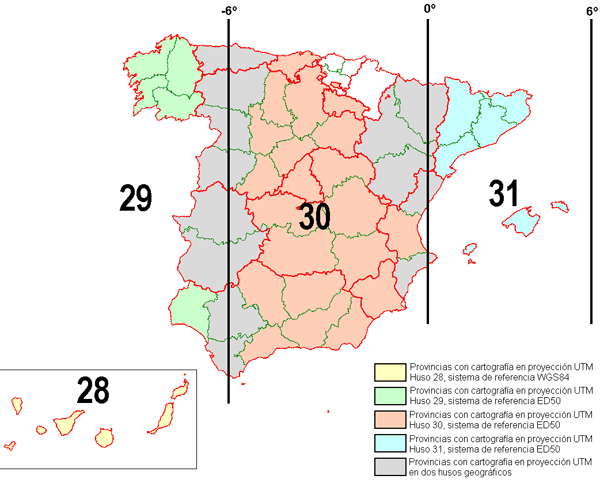
\includegraphics[width=9cm]{utm.png}
\caption{Mapa amb les zones UTM.}
\end{figure}
\newpage
Com es pot comprovar, la zona corresponent a Catalunya és la 31. Ara es necessita saber la lletra corresponent a la zona, que per a Catalunya és la 'T'.\\
Partint que per a la conversió, qualsevol coordenada dins de Catalunya tindrà com a zona la 31T, ja es pot fer servir una llibreria que ens permetrà la conversió de forma automàtica sense majors complicacions. S'utilitzarà la llibreria \emph{UTM}, i més concretament la seva funció to latlon().

\begin{figure}[!htbp]
\begin{verbatim}
coordenades = utm.to_latlon(item['utmX'],item['utmY'],31,'T')
item['lat'] = coordenades[0]
item['lon'] = coordenades[1]
\end{verbatim}
\caption{Conversió entre coordenades UTM i latitud/longitud.}
\end{figure}
Aquesta funció, com es pot veure a la figura anterior, retorna un vector amb primer el valor de la latitud, i després el corresponent a la longitud.\\ \\
Una vegada ja es tenen totes les dades que es desitgen pel projecte, es recorre tot el fitxer .xlsx que conté la informació de l'ICC i per cada fila es van agafant els valors especificats anteriorment. Es fa la conversió de les coordenades, i finalment cada valor es guarda a la base de dades amb l'\emph{insert} especificat anteriorment.
\newpage
\subsection*{Base de dades de ciutats de tot el món}
El treball es centra en una base de dades de notícies escrites en català i d'àmbit nacional, és per això que s'ha fet especial èmfasi en cobrir el territori català amb detall, però a nivell mundial s'ha optat per considerar només les ciutats més poblades.\\
Trobat una base de dades fiable i que reunís els requisits demanats consistia en tenir informació sobre les coordenades de cada ciutat, i a més informació sobre la seva població, ja que sinó no se'n podria determinar quina ciutat és suficientment important per a ésser considerada.\\ \\
La base de dades que s'ha escollit, ha estat la que manté geonames.org. Conté informació que es va actualitzant dia a dia, ja que tot i que el nucli d'aquesta informació prové de fonts oficials,  pot contenir errors i una comunitat activa de tot el món la va actualitzant i millorant. Aquesta base de dades és de lliure accés i ús sota una llicència Creative Commons.\\
La pàgina per accedir a les descàrregues de la base de dades, així com altres fitxers d'informació geogràfica diversa, es troba en el següent enllaç:

\begin{quote}
http://download.geonames.org/export/dump/
\end{quote}
Si observem els diferents fitxers que se'ns facilita a l'enllaç, podrem comprovar com n'hi ha de diferents tipus. Els fitxers que es poden trobar són:
\begin{itemize}
\item \textbf{XX.zip}: Conté informació per cada país, on XX correspon al seu codi ISO.
\item \textbf{allCountries.zip}: Tots els països en un sol fitxer.
\item \textbf{cities1000.zip}: Totes les ciutats amb una població major a 1000 habitants.
\item \textbf{cities5000.zip}: Totes les ciutats amb una població major a 5000 habitants.
\item \textbf{cities15000.zip}: Totes les ciutats amb una població major a 15000 habitants o capitals.
\item \textbf{alternateNames.zip}: Conté dos fitxers: el primer que conté els noms alternatius d'una ciutat (i.e.: el nom de la ciutat en diferents idiomes, noms alternatius d'una ciutat,...); el segon, és un fitxer que conté les referències entre els codis ISO i l'idioma que representen (i.e.: el català està representat amb el codi CA o CAT)
\item \textbf{admin1CodesASCII.txt}: Codis que fan referència a regions administratives en codificació ASCII.
\item \textbf{admin2Codes.txt}: Codis que fan referència a regions administratives en codificació UTF-8.
\item \textbf{iso-languagecodes.txt}: Codis ISO dels diferents idiomes. És el mateix fitxer inclòs dins del fitxer zip alternateNames.zip.
\item \textbf{featureCodes.txt}: Nom i descripció d'una característica. (i.e.: per a una entitat política es representa de la següent forma: "\emph{A.PCL	political entity}").
\item \textbf{timeZones.txt}: Informació sobre les hores de cada capital d'estat, concretament el desplaçament horari respecte DST i respecte el meridià de Greenwich.
\item \textbf{countryInfo.txt}: Informació diversa sobre cada país, com per exemple els codis postals o els idiomes oficials.
\item \textbf{...-<date>.txt}: Conté informació sobre les modificacions i eliminacions respecte l'anterior versió en cada un dels fitxers.
\item \textbf{Altres}: Hi ha altres fitxers que contenen informació com per exemple els autors de les modificacions.
\end{itemize}
Com s'ha mencionat anteriorment, es desitjarà mantenir una base de dades amb les ciutats més importants, i tal com podem veure hi ha fitxers ordenats per la població de les ciutats. En aquest cas, s'utilitzarà la base de dades amb ciutats que tenen una població superior als 15.000 habitants, per tant el primer fitxer a tenir en compte serà cities15000.zip i el fitxer alternateNames.zip per a poder agafar de cada ciutat el seu nom en català.\\

\subsubsection*{Obtenció}

\subsubsection*{Neteja}

\subsection*{Base de dades de notícies}

\subsubsection*{Obtenció}

\subsubsection*{Neteja}

\subsection{Obtenció de localitats en un text}

\subsection{Obtenció de les coordenades d'una localitat}

\subsection{Formatació de les dades per a CartoDB}

\subsection{Aplicació de l'algorisme DBScan}

\subsection{Visualització de les dades}

\subsection{Divulgació dels resultats}


\newpage

\section{Metodologia i resultats}
Agile??
desenvolupament iteratiu, avaluació, limitacions (producció i feedback usuaris)\\
Metodologia es refereix a com has organitzat el desenvolupament: has fet servir GitHub, aproximacions successives a la solució, altres tècniques de soft engineering que hagis fet servir, com avalues les solucions, etc.

\subsection{Metodologia}
\subsection{Resultats}

\newpage

\section{Concordança de resultats i objectius}

\newpage

\section{Conclusions}

Bla bla

\normalfont

\newpage

\begin{thebibliography}{25}
\bibitem{} Cohen, M.: TextGrounder: state of the art
\newline \texttt{https://mcohenlab.wordpress.com/textgrounder/}
\bibitem{} The Google Geocoding API
\newline \texttt{https://developers.google.com/maps/documentation/geocoding/}
\bibitem{} IBM Developer Networks: ¿Qué es Big Data?
\newline \texttt{https://www.ibm.com/developerworks/ssa/local/im/que-es-big-data/}
\bibitem{} Yahoo BOSS Geo Services: Overview
\newline \texttt{https://developer.yahoo.com/boss/geo/}
\bibitem{} Repositori GITHUB del projecte CLAVIN
\newline \texttt{https://github.com/Berico-Technologies/CLAVIN}
\bibitem{} Repositori BitBucket del projecte TextGrounder
\newline \texttt{https://bitbucket.org/utcompling/textgrounder/}
\bibitem{} PyPI - the Python Package Index
\newline \texttt{https://pypi.python.org/}
\bibitem{} MongoDB
\newline \texttt{https://www.mongodb.com/}


\bibitem{pari} Batut, C.; Belabas, K.; Bernardi, D.; Cohen, H.; Olivier, M.: User's guide to \textit{PARI-GP},  \newline \texttt{pari.math.u-bordeaux.fr/pub/pari/manuals/2.3.3/users.pdf}, 2000.
\bibitem{cw} Chen, J. R.; Wang, T. Z.: On the Goldbach problem, \textit{Acta Math. Sinica}, 32(5):702-718, 1989.
\bibitem{desh} Deshouillers, J. M.: Sur la constante de $\check{\text{S}}\text{nirel}^{\prime} \text{man}$, \textit{Séminaire Delange-Pisot-Poitou, 17e année: (1975/76), Théorie des nombres: Fac. 2, Exp. No.} G16, pàg. 6, Secràtariat Math., Paris, 1977.

\end{thebibliography}
\end{document} 

